\documentclass{beamer}

\usepackage{listings}
\usepackage{hyperref}
\usepackage{color}
\usepackage[utf8]{inputenc}
\usetheme{Madrid}
\setbeamersize{text margin left=0.1\textwidth,text margin right=0.1\textwidth}
\setbeamertemplate{section in toc}{\inserttocsection}
\lstset{language=python,
        keywordstyle=\color{red},
        basicstyle=\ttfamily,
        basicstyle=\small,
        frame = single,
        framexleftmargin=15pt,
        numbers=left,
        numberstyle=\small,
        numbersep=5pt,
        xleftmargin=0.05\textwidth,
        columns=fullflexible}

%Information to be included in the title page:
\title{Object Oriented Programming}
\author{Cary Goltermann}
\institute{Galvanize}
\date{2016}

 \AtBeginSubsection[]
{
  \begin{frame}
    \frametitle{Overview}
    \tableofcontents[currentsection,currentsubsection]
  \end{frame}
}

\begin{document}

\frame{\titlepage}

\begin{frame}
  \frametitle{Overview}
  \tableofcontents[]
\end{frame}

\section{OOP}
\subsection{Motivation}
\begin{frame}
  \frametitle{Coding Concerns}
  Much of what we are going to talk about today is concerned with the overarching topic of good software engineering practices. \vspace{4mm}

  \textbf{When we write code we are striving for it to be:}

  \vspace{4mm}
  \begin{itemize}
    \item Easy to maintain and modify
    \begin{itemize}
      \item Easy to understand
      \item Easy to use / re-use
      \item Split into logical components
    \end{itemize}
    \item Easy to test
  \end{itemize}
\end{frame}

\begin{frame}
  \frametitle{What is OOP?}
  Object oriented programming is a paradigm that allows us to model real-world ideas as ``objects'' in code. These objects have data and associated actions that can be done with that data. \vspace{4mm}
  \pause

  In this way a programs can be built up by defining objects and relationships between those objects. \vspace{4mm}
  \pause

    This model is quite popular for many reasons, but one of the main ones that proponents cite is that programming in this way models that the way that we think about the world, as things with relationships.
\end{frame}

\begin{frame}
  \frametitle{What is a Program?}
  A program is a set of instructions, \textbf{behavior}, that when performed on some data, \textbf{state}, results in some desired outcome. E.g. a calculation being performed or webpage rendered. \vspace{5mm}

  \begin{center}
  Program = State + Behavior
\end{center}
\end{frame}

\subsection{Definition}
\begin{frame}
  \frametitle{OOP - Formalization}
  OOP originated from a desire to have a way to program that mirrors how humans label, interpret and interact with the physical world. \vspace{4mm}

  In this way the state and behavior that make up a program are collected into \textbf{objects} and \textbf{classes}.
\end{frame}

\begin{frame}
  \frametitle{Objects}
  An \textbf{object} is a single entity containing: \vspace{4mm}

  \begin{description}
    \item[State] Variable(s), representing some data.
    \item[Behavior] Action(s), defining ways to interact with the state. 
  \end{description} \vspace{5mm}
  \pause
  
  \begin{columns}
    \column{0.7\textwidth}
    \begin{block}{Example: Blender}
      \begin{description}
        \item[State] Plugged in, On, Speed
        \item[Behavior] Plug in, Blend, Change Speed
      \end{description}
    \end{block}
    \column{0.3\textwidth}
      \vspace{3mm}
      \centering
      \includegraphics[width=\textwidth]{images/blender.jpg}
    \end{columns}
\end{frame}

\begin{frame}
  \frametitle{Classes}
  A \textbf{class} is a meta-concept that describes how an object operates. You can think of it like a blueprint for an object. In this way an object is a single realization, or \textbf{instance}, of a class. \vspace{4mm}
  \pause

  In this way the nature of the state and behavior that an object can have is specified in this blueprint, when the class for it is defined. \vspace{2mm}
\end{frame}

\subsection{Terminology}
\begin{frame}
  \frametitle{Attributes}
  Every object has a group of attributes. These attributes are where the data, the state, of the object resides. You can think of the data in an object's attributes as being "owned" by that object. \vspace{6mm}
  \pause
  
  \begin{columns}
    \column{0.5\textwidth}
    \begin{block}{Example: Blender Attributes}
      \begin{itemize}
        \item \texttt{plugged\_in} $\rightarrow$ Bool
        \item \texttt{on} $\rightarrow$ Bool
        \item \texttt{speed} $\rightarrow$ Int
      \end{itemize}
    \end{block}
    \pause
    \column{0.5\textwidth}
    \vspace{2mm}

    The value of these attributes defines the object's state. To access that state that lives on the object we use \textit{dot notation}. E.g. \texttt{my\_blender.speed}.
  \end{columns}
\end{frame}

\begin{frame}
  \frametitle{Methods}
  In addition to the attributes which store an object's state, every object has a set of \textbf{methods} that define the object's behavior. A method is simply a procedure that has access to an object's state. \vspace{2mm}
 \pause 

 Frequently, methods will change its object state, in fact, methods are the de facto correct way to interact with an object's state. \vspace{4mm}
  \pause

  \begin{block}{Example: Blender Methods}
    \begin{itemize}
      \item \texttt{plug()} $\rightarrow$ Changes \texttt{plugged\_in} attribute.
      \item \texttt{toggle\_power()} $\rightarrow$ Changes \texttt{on} attribute.
      \item \texttt{set\_speed(speed)} $\rightarrow$ Changes \texttt{speed} attribute to specified int.
    \end{itemize}
  \end{block}
\end{frame}

\section{OOP - Tenets}
\begin{frame}
  \frametitle{Tenets}
  In object oriented programming there are three (and a half) overarching ideas that guide the way that we about making classes. \vspace{5mm}

  \begin{itemize}
    \item Encapsulation
    \item Inheritance - but we'll mostly talk about Composition
    \item Polymorphism
  \end{itemize}
\end{frame}

\subsection{Encapsulation}
\begin{frame}
  \frametitle{Encapsulation}
  Expands the concept of abstraction that we take advantage of when writing functions to include both the: \textbf{state} and \textbf{behavior} that we deal with when working with objects. \vspace{4mm}
  \pause

  This means that not only are the details of how the behavior are implemented, but also, the details about how are state is being stored.
\end{frame}

\begin{frame}
  \frametitle{Encapsulation Benefits}
  The implications of encapsulation make working with classes easy in a number of ways: \vspace{4mm}

  \begin{enumerate}
    \item<1-> When using the class we don't have to worry about the details about how any of the state is being stored, or how the behavior is being implemented.
    \item<2-> This lack of concern makes it so that the implementations can changes without any user ever knowing, so long as the interface remains unchanged.
  \end{enumerate}
\end{frame}

\begin{frame}[fragile]
  \frametitle{Encapsulation Example}
  \begin{lstlisting}
  In [1]: from collections import Counter

  In [2]: c = Counter('Hello')
 
  In [3]: c
  Out[3]: Counter({'e': 1,'h': 1,'l': 2,'o': 1})

  In [4]: c.most_common()
  Out[4]: [('l', 2), ('o', 1), ('e', 1), ('h', 1)]
  \end{lstlisting}
  \vspace{5mm}
  \pause
  How does \texttt{most\_common()} work? For that matter, how is the data in a Counter stored? Does it matter that we don't actually know?
\end{frame}

\subsection{Composition}
\begin{frame}
  \frametitle{Composition}
  When building up our own classes we want to strive to have each class concerned with a single specific concept. However, frequently we'll find that we want to make classes that encompass complicated ideas. \vspace{4mm}

  In these circumstances we can have the attributes of our complicated class be instances of another class. We call this class \textbf{composition}, in that we are composing the complicated class from other, specifically focused, hopefully simpler classes.
\end{frame}

\begin{frame}
  \frametitle{Example Class - Deck of Cards}
  What are the objects that we might want to make if we were codifying the concept of a deck of cards? \pause \textbf{Card} \texttt{\&} \textbf{Deck}? \vspace{5mm}
  \pause

  The language we use to describe this relationship is that a Deck \textbf{has-a} Card, many of them in fact. \vspace{1mm}
\end{frame}

\begin{frame}[fragile]
  \frametitle{Example Class Cont.}
  \begin{lstlisting}
  import random

  class Card(object):
      def __init__(self, number, suit):
          self.suit = suit
          self.number = number

  class Deck(object):
      def __init__(self):
          self.cards = []
          for num in ['2', '3', '4', '5', '6', '7', '8',
                      '9', '10', 'J', 'Q', 'K', 'A']:
              for suit in 'cdhs':
                  self.cards.append(Card(num, suit))
  \end{lstlisting}
\end{frame}

\begin{frame}[fragile]
  \frametitle{Example Class Cont.}
  \begin{lstlisting}
    ...
      def shuffle(self):
          random.shuffle(self.cards)

      def draw_card(self):
          if not self.isempty():
              return self.cards.pop()

      def add_cards(self, cards):
          self.cards.extend(cards)

      def isempty(self):
          return self.cards == []
  \end{lstlisting}
\end{frame}

\begin{frame}
  \frametitle{Built-in Operations}
  When we write custom classes we frequently want to enable instances of them to interact with built-in language operations so that we can use them like built in classes. \vspace{4mm}
  
  Consider that we can compare strings with $`brain` <\ `pinky`$, and we can find the length of containers with $len()$. \vspace{4mm}
  \pause

  \begin{block}{}
    The functionality that we desire is known as operator overloading, and in Python it is available to us via \textbf{magic methods}.
  \end{block}
\end{frame}

\begin{frame}[fragile]
  \frametitle{Magic Methods}
  Magic methods are any methods that begin and end with a double underscore (the double underscore convention is exclusively reserved for magic methods). The functionality they afford us enable interaction with built-in language operations. \vspace{5mm}
  
  {\large Example: Length and Stringing}

  \begin{lstlisting}
  class Deck(object):
    ...
      def __len__(self):
          return len(self.cards)
  \end{lstlisting}
  \pause
  \begin{lstlisting}
  class Card(object):
    ...
      def __str__(self):
          return '{}{}'.format(self.number, self.suit)
  \end{lstlisting}
\end{frame}

\begin{frame}[fragile]
  \frametitle{Two Object Magic Method Example}
  When we work with operations that involve two objects we need to have a way to access information about both. Python handles this by passing a reference to each of the objects to the magic method that implements the operation's functionality. Convention is to use the names \textbf{self} (per the usual) and \textbf{other}. \vspace{2mm}
  \pause

  \begin{lstlisting}
  class Card(object):
    ...
      def __cmp__(self, other):
          return cmp(self.number, other.number)
  \end{lstlisting}

  \textit{Note: self.number and other.number may be characters.} \vspace{2mm}

  The {\color{blue}\href{https://docs.python.org/2/library/functions.html#cmp}{cmp()}} function is built into Python. Returns $-1$ if the first is less than the second, $1$ if the reverse is true, and $0$ if they are equal.
\end{frame}

\subsection{Polymorphism}
\begin{frame}
  \frametitle{Polymorphism}
  Having the abstraction of a class' behavior span multiple classes of a similar type is frequently a desirable trait. This next level of abstraction is referred to as \textbf{polymorphism}, and is formally defined as: \vspace{5mm}

  \begin{block}{Polymorphism}
    The provision of a single interface for objects of different classes.
  \end{block}
\end{frame}

\subsection{Inheritance}
\begin{frame}
  \frametitle{Inheritance}
  Sometimes when we are designing classes we find that there exists a common structure and functionality that underlies multiple classes. In these situations we would like to abstract out these commonalities, and have a process by which we share that functionality. \vspace{4mm}
  \pause

  Inheritance defines a framework in which a class, the child class, can be based off of another class, the parent class. When the child inherits from the parents the functionality defined on the parent class is accessible to the child for free. This process of inheriting allows for effective code reuse amongst like classes.
\end{frame}

\begin{frame}
  \frametitle{Inheritance Example: Is-a Relationship}
  Say we were trying to model some fruit that we frequently eat at home: bananas, oranges, and apples. What do we think the underlying structure and functionality of these classes might be? What would we call it? \pause \textbf{Fruit} - you can eat fruit, it has a weight, and it must be grown. \vspace{2mm}
  \pause
  \begin{center}
    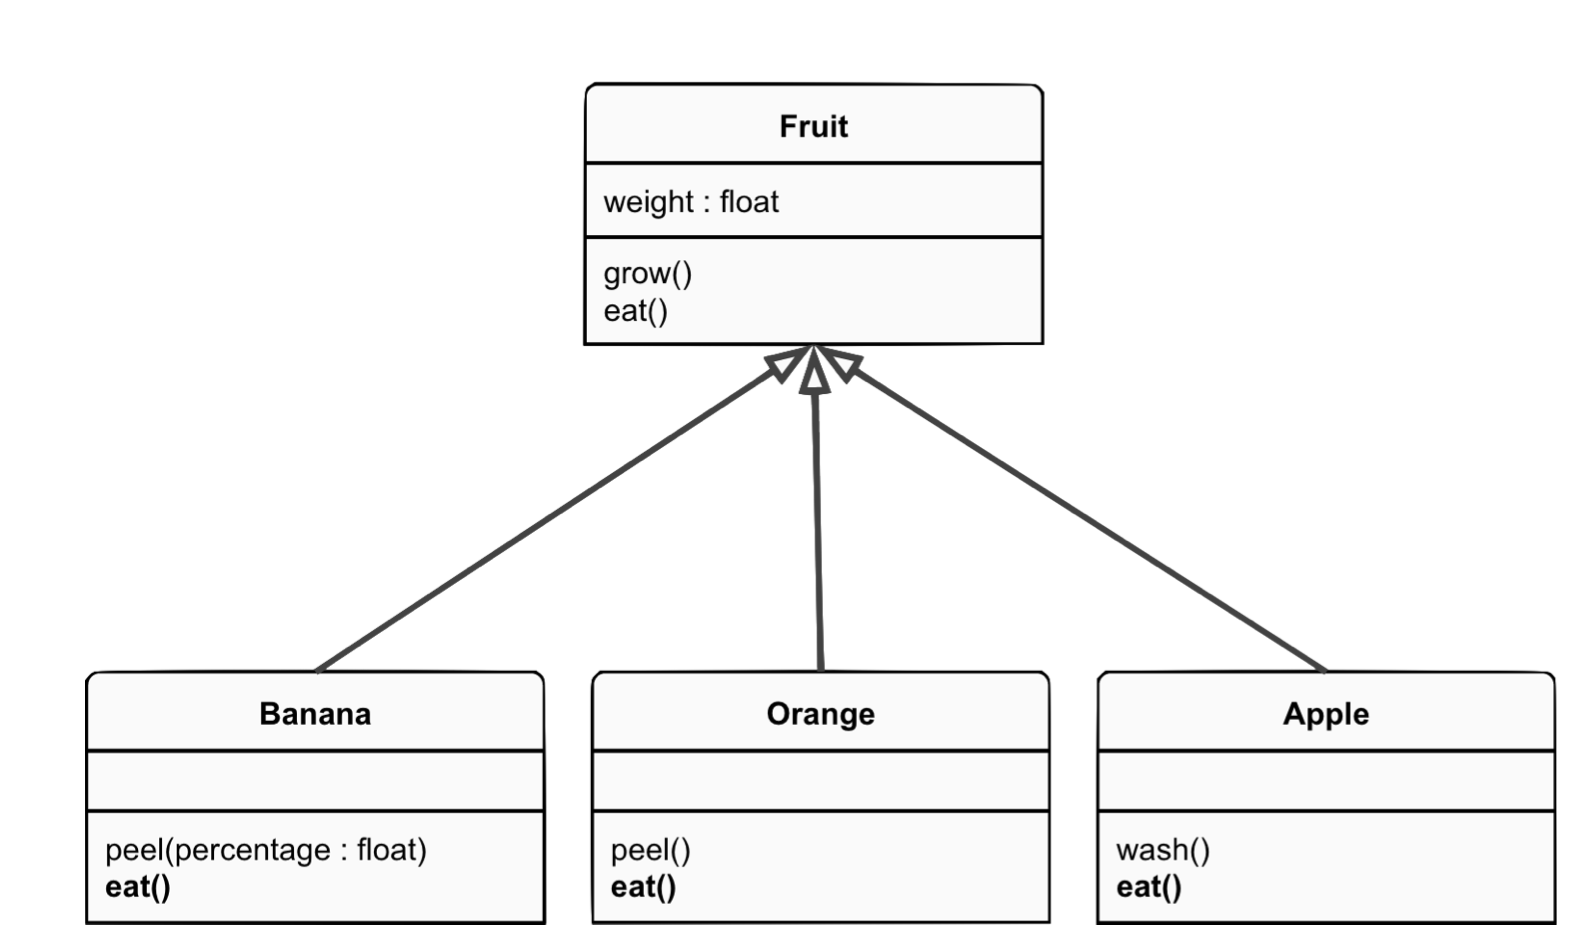
\includegraphics[width=0.8\textwidth]{images/inheritance.png}
  \end{center}
\end{frame}

\end{document}
